% Options for packages loaded elsewhere
\PassOptionsToPackage{unicode}{hyperref}
\PassOptionsToPackage{hyphens}{url}
\PassOptionsToPackage{dvipsnames,svgnames,x11names}{xcolor}
%
\documentclass[
  letterpaper,
  DIV=11,
  numbers=noendperiod]{scrartcl}

\usepackage{amsmath,amssymb}
\usepackage{iftex}
\ifPDFTeX
  \usepackage[T1]{fontenc}
  \usepackage[utf8]{inputenc}
  \usepackage{textcomp} % provide euro and other symbols
\else % if luatex or xetex
  \usepackage{unicode-math}
  \defaultfontfeatures{Scale=MatchLowercase}
  \defaultfontfeatures[\rmfamily]{Ligatures=TeX,Scale=1}
\fi
\usepackage{lmodern}
\ifPDFTeX\else  
    % xetex/luatex font selection
\fi
% Use upquote if available, for straight quotes in verbatim environments
\IfFileExists{upquote.sty}{\usepackage{upquote}}{}
\IfFileExists{microtype.sty}{% use microtype if available
  \usepackage[]{microtype}
  \UseMicrotypeSet[protrusion]{basicmath} % disable protrusion for tt fonts
}{}
\makeatletter
\@ifundefined{KOMAClassName}{% if non-KOMA class
  \IfFileExists{parskip.sty}{%
    \usepackage{parskip}
  }{% else
    \setlength{\parindent}{0pt}
    \setlength{\parskip}{6pt plus 2pt minus 1pt}}
}{% if KOMA class
  \KOMAoptions{parskip=half}}
\makeatother
\usepackage{xcolor}
\setlength{\emergencystretch}{3em} % prevent overfull lines
\setcounter{secnumdepth}{-\maxdimen} % remove section numbering
% Make \paragraph and \subparagraph free-standing
\makeatletter
\ifx\paragraph\undefined\else
  \let\oldparagraph\paragraph
  \renewcommand{\paragraph}{
    \@ifstar
      \xxxParagraphStar
      \xxxParagraphNoStar
  }
  \newcommand{\xxxParagraphStar}[1]{\oldparagraph*{#1}\mbox{}}
  \newcommand{\xxxParagraphNoStar}[1]{\oldparagraph{#1}\mbox{}}
\fi
\ifx\subparagraph\undefined\else
  \let\oldsubparagraph\subparagraph
  \renewcommand{\subparagraph}{
    \@ifstar
      \xxxSubParagraphStar
      \xxxSubParagraphNoStar
  }
  \newcommand{\xxxSubParagraphStar}[1]{\oldsubparagraph*{#1}\mbox{}}
  \newcommand{\xxxSubParagraphNoStar}[1]{\oldsubparagraph{#1}\mbox{}}
\fi
\makeatother


\providecommand{\tightlist}{%
  \setlength{\itemsep}{0pt}\setlength{\parskip}{0pt}}\usepackage{longtable,booktabs,array}
\usepackage{calc} % for calculating minipage widths
% Correct order of tables after \paragraph or \subparagraph
\usepackage{etoolbox}
\makeatletter
\patchcmd\longtable{\par}{\if@noskipsec\mbox{}\fi\par}{}{}
\makeatother
% Allow footnotes in longtable head/foot
\IfFileExists{footnotehyper.sty}{\usepackage{footnotehyper}}{\usepackage{footnote}}
\makesavenoteenv{longtable}
\usepackage{graphicx}
\makeatletter
\newsavebox\pandoc@box
\newcommand*\pandocbounded[1]{% scales image to fit in text height/width
  \sbox\pandoc@box{#1}%
  \Gscale@div\@tempa{\textheight}{\dimexpr\ht\pandoc@box+\dp\pandoc@box\relax}%
  \Gscale@div\@tempb{\linewidth}{\wd\pandoc@box}%
  \ifdim\@tempb\p@<\@tempa\p@\let\@tempa\@tempb\fi% select the smaller of both
  \ifdim\@tempa\p@<\p@\scalebox{\@tempa}{\usebox\pandoc@box}%
  \else\usebox{\pandoc@box}%
  \fi%
}
% Set default figure placement to htbp
\def\fps@figure{htbp}
\makeatother

\usepackage{booktabs}
\usepackage{longtable}
\usepackage{array}
\usepackage{multirow}
\usepackage{wrapfig}
\usepackage{float}
\usepackage{colortbl}
\usepackage{pdflscape}
\usepackage{tabu}
\usepackage{threeparttable}
\usepackage{threeparttablex}
\usepackage[normalem]{ulem}
\usepackage{makecell}
\usepackage{xcolor}
\KOMAoption{captions}{tableheading}
\makeatletter
\@ifpackageloaded{caption}{}{\usepackage{caption}}
\AtBeginDocument{%
\ifdefined\contentsname
  \renewcommand*\contentsname{Table of contents}
\else
  \newcommand\contentsname{Table of contents}
\fi
\ifdefined\listfigurename
  \renewcommand*\listfigurename{List of Figures}
\else
  \newcommand\listfigurename{List of Figures}
\fi
\ifdefined\listtablename
  \renewcommand*\listtablename{List of Tables}
\else
  \newcommand\listtablename{List of Tables}
\fi
\ifdefined\figurename
  \renewcommand*\figurename{Figure}
\else
  \newcommand\figurename{Figure}
\fi
\ifdefined\tablename
  \renewcommand*\tablename{Table}
\else
  \newcommand\tablename{Table}
\fi
}
\@ifpackageloaded{float}{}{\usepackage{float}}
\floatstyle{ruled}
\@ifundefined{c@chapter}{\newfloat{codelisting}{h}{lop}}{\newfloat{codelisting}{h}{lop}[chapter]}
\floatname{codelisting}{Listing}
\newcommand*\listoflistings{\listof{codelisting}{List of Listings}}
\makeatother
\makeatletter
\makeatother
\makeatletter
\@ifpackageloaded{caption}{}{\usepackage{caption}}
\@ifpackageloaded{subcaption}{}{\usepackage{subcaption}}
\makeatother

\usepackage{bookmark}

\IfFileExists{xurl.sty}{\usepackage{xurl}}{} % add URL line breaks if available
\urlstyle{same} % disable monospaced font for URLs
\hypersetup{
  pdftitle={UFC Analysis - IDS 702 Final Project},
  pdfauthor={Arko Bhattacharya, Eric Ortega Rodriguez, Mu Niu, Nruta Choudhari},
  colorlinks=true,
  linkcolor={blue},
  filecolor={Maroon},
  citecolor={Blue},
  urlcolor={Blue},
  pdfcreator={LaTeX via pandoc}}


\title{UFC Analysis - IDS 702 Final Project}
\author{Arko Bhattacharya, Eric Ortega Rodriguez, Mu Niu, Nruta
Choudhari}
\date{2024-12-15}

\begin{document}
\maketitle


\subsection{Abstract}\label{abstract}

Understanding the impact of physical attributes, such as reach, and
tactical strategies, such as submission attempts, is critical for
improving performance and outcomes in mixed martial arts (MMA). This
study examined the relationship between fighter reach and the total
number of strikes landed during a fight. Additionally, it investigated
the role of submission attempts in predicting fight outcomes, using a
dataset of fights from the Ultimate Fighting Championship (UFC), the
leading global MMA promotion. The dataset included UFC fights from March
2010 to the most recent event in 2024.

Linear regression with log-transformed variables revealed significant
interactions between reach and weight classes, such as Flyweight and
Featherweight, highlighting that reach impacts striking performance
differently across divisions. Main effects were also observed for weight
classes like Flyweight and Women's Strawweight. Logistic regression
showed that submission attempts significantly influenced fight outcomes,
with red corner attempts positively associated with winning odds and
blue corner attempts negatively associated. Both predictors had p-values
below 0.05. Model diagnostics, including residual analysis and
multicollinearity checks, confirmed the validity of the findings.

These results underscore the tactical importance of physical attributes
and strategic maneuvers in UFC fights, providing insights to optimize
training and fight preparation. Future research could explore additional
predictors, such as fighter skill level and strategy, or advanced
modeling techniques to deepen understanding of combat sports
performance.

\subsection{Introduction}\label{introduction}

The Ultimate Fighting Championship (UFC) is the world's leading mixed
martial arts (MMA) promotion, known for bringing together elite fighters
from diverse combat sports backgrounds. Founded in 1993, the UFC has
grown into a global phenomenon, hosting events worldwide that showcase
athletes competing in disciplines such as boxing, wrestling, Muay Thai,
Brazilian Jiujitsu, and judo. UFC fights take place in a distinct
eight-sided cage, known as the Octagon, where fighters test their skills
in striking, grappling, and overall strategy under a unified set of
rules. The sport has evolved significantly over the years, introducing
standardized weight classes, safety regulations, and scoring systems to
ensure competitive fairness and fighter safety.

This project examines UFC performances using data on UFC fights from
2010 to the present (last updated in November, 2024). The data, sourced
from Kaggle, includes key fighter metrics, fight outcomes, betting odds,
and performance indicators such as strikes landed and submission
attempts. By leveraging this dataset, we aim to analyze factors
influencing fight outcomes and performances.

Our research questions are:

\begin{enumerate}
\def\labelenumi{\arabic{enumi}.}
\tightlist
\item
  How does the reach of the fighter relate to the total number of
  strikes landed during a fight?
\item
  Is the fight outcome associated with the number of submission attempts
  made by a fighter?
\end{enumerate}

These questions are worth exploring because they provide a deeper
understanding of UFC performance dynamics. For instance, examining the
relationship between a fighter's reach and the total number of strikes
landed can underscore the tactical performance of physical attributes in
effective striking. Similarly, analyzing the association between fight
outcomes and submission attempts can shed light on the strategic role of
grappling in securing victories.

The findings from this analysis offer valuable insights for fighters,
coaches, and analysts, helping optimize training strategies, improve
fight preparation, and enhance understanding of opponents' strengths and
weaknesses.

\subsection{Methods}\label{methods}

\paragraph{Data and Preprocessing}\label{data-and-preprocessing}

The dataset was obtained from Kaggle, a widely recognized platform for
sharing datasets and data science resources. Each row of the dataset
refers to an individual bout, which refers to an individual match
between two fighters. This includes data on fighter attributes such as
height, weight, reach, stance, and age, as well as fight statistics like
strikes landed, significant strikes, takedowns, submission attempts, and
knockdowns. Additionally, it documents fight outcomes, including the
winner, method of victory (e.g., knockout, submission, decision), the
round in which the fight ended, and the total duration of the fight.

The dataset contains 6,478 rows across 118 columns, with several
variables containing missing values. During preprocessing, columns with
over 6,000 missing values were dropped due to their lack of significance
and the infeasibility of imputation. Other columns had a smaller
proportion of missing values, and rows with missing values in key
variables (e.g., strikes landed, reach, and weight class) were removed.
This resulted in a final dataset with 4,895 rows. Most of the missing
values were concentrated in performance metrics, such as submission
attempts or specific strike statistics.

In UFC, fighters are assigned to either the red corner or the blue
corner, which indicates their position in the Octagon and helps
differentiate between competitors. For the first research question, the
dataset was filtered to include the variables related to reach, weight
class, height, strikes landed and current win streak, ensuring that key
confounding variables were included. The data for fighters in the red
and blue corners were combined into a single dataframe to facilitate
analysis.

For the second research question, a new binary variable, Outcome was
created to indicate the winner. A value of 1 was assigned if the fighter
in the red corner won, and a value of 0 if the fighter in the blue
corner won. The model included variables such as submission attempts,
significant strikes landed, fight duration, and weight class to account
for both physical attributes and performance metrics. These variables
ensured a more comprehensive analysis of the factors influencing fight
outcomes while addressing potential confounders.

\paragraph{Model Fitting and
Evaluation}\label{model-fitting-and-evaluation}

To examine the relationship between a fighter's reach and the total
number of strikes landed during a fight, a Multiple Linear Regression
(MLR) model was utilized. The model included key predictors such as
logarithmic transformation of reach, logarithmic transformation of
height, win streak and weight class, with an interaction term between
the win streak and weight class to explore potential moderating effects.
Outliers and influential points were identified using Cook's distance,
and these were removed to improve model robustness. Diagnostics,
including residuals vs.~fitted plots, were performed to assess linearity
and homoscedasticity, while Variance Inflation Factor (VIF) was used to
evaluate multicollinearity. Model performance was measured using the
R-squared value.

For the second research question, a logistic regression model was
employed to predict fight outcomes (binary: win or loss) using
submission attempts, reach, significance strikes, fight duration, and
weight class as predictors. The model was refined using stepwise
selection to identify the most significant predictors, and diagnostics
such as Cook's distance, leverage, and deviance residuals were used to
detect and remove influential points. The final logistic regression
model included key predictors such as logarithmic transformations of
submission attempts, logarithmic transformation of reach, logarithmic
transformation of significant strikes landed, and logarithmic
transformation of fight duration. Model performance was evaluated using
the area under the receiver operating characteristic curve (ROC curve),
and diagnostic plots were generated to assess the model's fit.

All the analyses were conducted in R.

\subsection{Results}\label{results}

\paragraph{Research Question 1: How does the reach of the fighter relate
to the total number of strikes landed during a
fight?}\label{research-question-1-how-does-the-reach-of-the-fighter-relate-to-the-total-number-of-strikes-landed-during-a-fight}

To explore the relationship between a fighter's reach and the number of
strikes landed, we began by computing summary statistics for key
variables: Reach, Weight Class, Height, Win Streak, and Average
Significant Strikes Landed. Continuous variables are reported as means
with standard deviations, while categorical variables are summarized by
counts and percentages. These statistics provide as foundation for
understanding the data before modelling.

\begin{longtable}[]{@{}
  >{\centering\arraybackslash}p{(\linewidth - 10\tabcolsep) * \real{0.2738}}
  >{\centering\arraybackslash}p{(\linewidth - 10\tabcolsep) * \real{0.0714}}
  >{\centering\arraybackslash}p{(\linewidth - 10\tabcolsep) * \real{0.1667}}
  >{\centering\arraybackslash}p{(\linewidth - 10\tabcolsep) * \real{0.1548}}
  >{\centering\arraybackslash}p{(\linewidth - 10\tabcolsep) * \real{0.1548}}
  >{\centering\arraybackslash}p{(\linewidth - 10\tabcolsep) * \real{0.1786}}@{}}
\caption{Summary Statistics by Weight Class}\tabularnewline
\toprule\noalign{}
\begin{minipage}[b]{\linewidth}\centering
WeightClass
\end{minipage} & \begin{minipage}[b]{\linewidth}\centering
N
\end{minipage} & \begin{minipage}[b]{\linewidth}\centering
Avg\_Reach
\end{minipage} & \begin{minipage}[b]{\linewidth}\centering
Avg\_Height
\end{minipage} & \begin{minipage}[b]{\linewidth}\centering
Avg\_Strikes
\end{minipage} & \begin{minipage}[b]{\linewidth}\centering
Median\_Streak
\end{minipage} \\
\midrule\noalign{}
\endfirsthead
\toprule\noalign{}
\begin{minipage}[b]{\linewidth}\centering
WeightClass
\end{minipage} & \begin{minipage}[b]{\linewidth}\centering
N
\end{minipage} & \begin{minipage}[b]{\linewidth}\centering
Avg\_Reach
\end{minipage} & \begin{minipage}[b]{\linewidth}\centering
Avg\_Height
\end{minipage} & \begin{minipage}[b]{\linewidth}\centering
Avg\_Strikes
\end{minipage} & \begin{minipage}[b]{\linewidth}\centering
Median\_Streak
\end{minipage} \\
\midrule\noalign{}
\endhead
\bottomrule\noalign{}
\endlastfoot
Bantamweight & 1015 & 174.7 ± 6 & 170.8 ± 4.3 & 21.2 ± 21.1 & 1
{[}0-2{]} \\
Catch Weight & 77 & 180.8 ± 10.1 & 176.6 ± 8.6 & 8.6 ± 11.4 & 1
{[}0-2{]} \\
Featherweight & 1118 & 179.7 ± 5.7 & 175.2 ± 5 & 22.3 ± 21.1 & 1
{[}0-2{]} \\
Flyweight & 523 & 170.4 ± 5.7 & 167 ± 4.3 & 20.3 ± 21.4 & 1 {[}0-2{]} \\
Heavyweight & 715 & 197.4 ± 7.2 & 190.7 ± 5.8 & 18.4 ± 17.4 & 1
{[}0-2{]} \\
Light Heavyweight & 757 & 194.3 ± 6.5 & 188.2 ± 4.3 & 21.4 ± 18.2 & 1
{[}0-2{]} \\
Lightweight & 1665 & 181.8 ± 5.6 & 177.2 ± 4.6 & 23.3 ± 19.2 & 1
{[}0-2{]} \\
Middleweight & 1188 & 190.6 ± 5.9 & 185 ± 4.3 & 19.5 ± 17.4 & 1
{[}0-2{]} \\
Welterweight & 1527 & 187.1 ± 6 & 181.8 ± 4.4 & 23.3 ± 19.3 & 1
{[}0-2{]} \\
Women's Bantamweight & 302 & 170.6 ± 5.3 & 169.3 ± 4.4 & 21.2 ± 24.8 & 1
{[}0-1{]} \\
Women's Featherweight & 35 & 174.6 ± 5.6 & 171.1 ± 6.1 & 6.9 ± 10.3 & 1
{[}0-1{]} \\
Women's Flyweight & 355 & 168.6 ± 5.8 & 166.5 ± 4 & 11.3 ± 19.1 & 1
{[}0-2{]} \\
Women's Strawweight & 458 & 162.1 ± 5.7 & 161.5 ± 4.6 & 22.6 ± 28.1 & 1
{[}0-2{]} \\
\end{longtable}

\pandocbounded{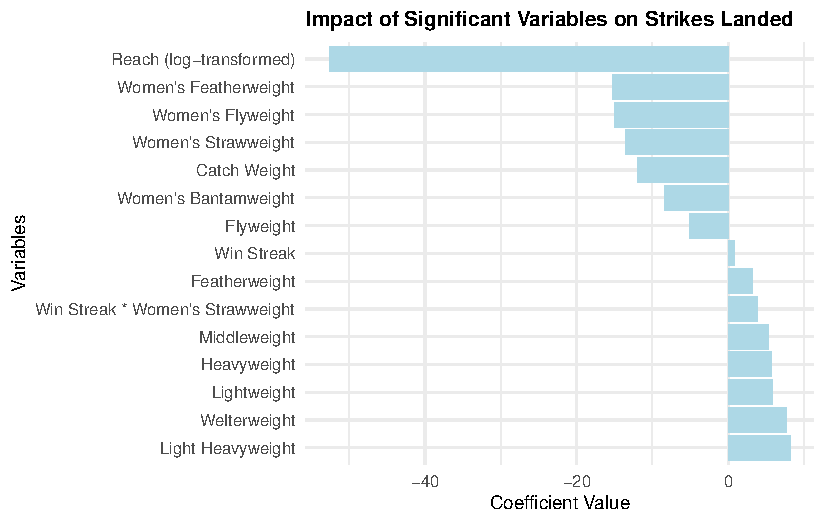
\includegraphics[keepaspectratio]{ufc_final_files/figure-pdf/unnamed-chunk-7-1.pdf}}

A multiple linear regression (MLR) model was applied to examine the
relationship between the average significant strikes landed and key
predictors, including log-transformed Reach, log-transformed Height, Win
Streak, and the interaction between Win Streak and Weight Class. The log
transformations for Reach and Height were performed to address
non-linearity and non-constant variance, which were highlighted in
diagnostic plots (see Appendix 1).

The adjusted \(R^2\)~value for the model was 0.068, suggesting that the
predictors explain approximately 6.8\% of the variability in average
significant strikes landed.

The analysis revealed several significant relationships between the
fighters' physical attributes and the number of significant strikes
landed. Notably, log-transformed Reach had a significant negative effect
on the number of strikes landed (\(\beta = -52.68, p < 0.001\)),
suggesting that reach increases, the average number of strikes landed
decreases. The Weight Class variable also showed significant effects
across divisions. Fighters in the Featherweight class landed more
strikes landed (\(\beta = 3.15, p = 0.001\)), while Flyweight fighters
landed fewer strikes (\(\beta = -5.12, p < 001\)). On the other hand,
Women's Flyweight fighters had a significant negative relationship with
strikes landed (\(\beta = -14.95, p < 0.001\)). In terms of interaction
effects, the model included interaction terms between Win Streak and
Weight Class, but most of these were not significant. However, there was
a marginally significant positive interaction observed for Women's
Strawweight (\(\beta = 3.88, p = 0.0008\)), suggesting that an
increasing win streak slightly positively impacts the number of strikes
landed in this weight class. Finally, the logarithm of the height
variable showed a weak, marginally significant negative relationship
with strikes landed (\(\beta = -15.59, p = 0.087\)), suggesting that
taller fighters might land fewer strikes on average, although the effect
is not strong. These findings underscore the complex interplay between a
fighter's physical characteristics, weight class, and performance
outcomes, with reach and weight class being the most influential factors
in predicting the number of strikes landed.

\pandocbounded{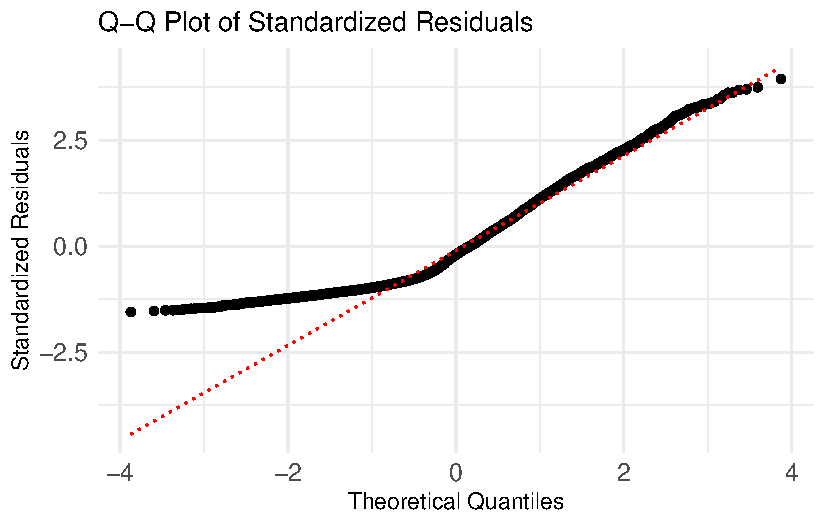
\includegraphics[keepaspectratio]{ufc_final_files/figure-pdf/unnamed-chunk-8-1.pdf}}

The initial multiple linear regression model violated the linearity
assumption, as indicated by the Q-Q plot in Appendix 1. To address this,
the outliers and influential values were identified and removed using
Cook's distance with the threshold set as \(\frac{4}{n}\), where n is
the total number of observations. After removing the influential points,
the model was re-evaluated, and the variables were log-transformed. This
iteration of the model proved to be a significant improvement from the
original, as evidenced by improved diagnostics and fit.

\begin{longtable}[]{@{}cccc@{}}
\caption{Variance Inflation Factor (VIF) and Adjusted
GVIF}\tabularnewline
\toprule\noalign{}
Variable & GVIF & Df & GVIF\_Adjusted \\
\midrule\noalign{}
\endfirsthead
\toprule\noalign{}
Variable & GVIF & Df & GVIF\_Adjusted \\
\midrule\noalign{}
\endhead
\bottomrule\noalign{}
\endlastfoot
Reach (log transformed) & 5.707 & 1 & 2.389 \\
Win Streak & 11.785 & 1 & 3.433 \\
Weight Class & 1301.455 & 12 & 1.348 \\
Height (log transformed) & 6.580 & 1 & 2.565 \\
Win Streak * Weight Class & 3430.027 & 12 & 1.404 \\
\end{longtable}

To assess multicollinearity, we calculated the Generalized Variance
Inflation Factor (GVIF) for each predictor, especially considering the
inclusion of categorical variables like Weight Class and their
interactions with Win Streak. The GVIF was adjusted using
\(GVIF^{\frac{1}{2 \cdot \text{df}}}\) to account for the degrees of
freedom of categorical variables and interaction terms, ensuring a more
accurate evaluation of multicollinearity. The results showed that most
predictors showed acceptable GVIF values, indicating no significant
multicollinearity. Although Weight Class had a high raw GVIF of 1301.45,
the adjusted GVIF was 1.35, indicating low multicollinearity. Overall,
the analysis confirmed that multicollinearity is not a significant
concern, allowing for reliable interpretation of the predictors.

\paragraph{Research Question 2: Is the fight outcome associated with the
number of submission attempts made by a
fighter?}\label{research-question-2-is-the-fight-outcome-associated-with-the-number-of-submission-attempts-made-by-a-fighter}

To explore the relationship between the number of submission attempts
and the fight outcome, we first computed summary statistics for key
variables: Submission Attempts, Weight Class, Reach, Significant Strikes
Landed, and Fight Time. The binary fight outcome is represented as 1 for
a Red win and 0 for a Blue win. Continuous variables, including
submission attempts, reach, significant strikes landed, and fight time,
are transformed using logarithmic transformations to account for
skewness. These transformations help in better understanding the
distribution and potential association with fight outcomes. Summary
statistics for these variables provide the necessary foundation for
further modeling.

\begin{longtable}[]{@{}
  >{\centering\arraybackslash}p{(\linewidth - 10\tabcolsep) * \real{0.2771}}
  >{\centering\arraybackslash}p{(\linewidth - 10\tabcolsep) * \real{0.0602}}
  >{\centering\arraybackslash}p{(\linewidth - 10\tabcolsep) * \real{0.2048}}
  >{\centering\arraybackslash}p{(\linewidth - 10\tabcolsep) * \real{0.1325}}
  >{\centering\arraybackslash}p{(\linewidth - 10\tabcolsep) * \real{0.1446}}
  >{\centering\arraybackslash}p{(\linewidth - 10\tabcolsep) * \real{0.1807}}@{}}
\caption{Summary Statistics by Weight Class}\tabularnewline
\toprule\noalign{}
\begin{minipage}[b]{\linewidth}\centering
WeightClass
\end{minipage} & \begin{minipage}[b]{\linewidth}\centering
N
\end{minipage} & \begin{minipage}[b]{\linewidth}\centering
Avg\_SubAttempts
\end{minipage} & \begin{minipage}[b]{\linewidth}\centering
Avg\_Reach
\end{minipage} & \begin{minipage}[b]{\linewidth}\centering
Avg\_SigStr
\end{minipage} & \begin{minipage}[b]{\linewidth}\centering
Avg\_FightTime
\end{minipage} \\
\midrule\noalign{}
\endfirsthead
\toprule\noalign{}
\begin{minipage}[b]{\linewidth}\centering
WeightClass
\end{minipage} & \begin{minipage}[b]{\linewidth}\centering
N
\end{minipage} & \begin{minipage}[b]{\linewidth}\centering
Avg\_SubAttempts
\end{minipage} & \begin{minipage}[b]{\linewidth}\centering
Avg\_Reach
\end{minipage} & \begin{minipage}[b]{\linewidth}\centering
Avg\_SigStr
\end{minipage} & \begin{minipage}[b]{\linewidth}\centering
Avg\_FightTime
\end{minipage} \\
\midrule\noalign{}
\endhead
\bottomrule\noalign{}
\endlastfoot
Bantamweight & 508 & 0.3 ± 0.3 & 5.2 ± 0 & 2.6 ± 1.1 & 6.3 ± 0.9 \\
Catch Weight & 39 & 0.5 ± 0.5 & 5.2 ± 0.1 & 1.9 ± 0.7 & 6.3 ± 0.8 \\
Featherweight & 562 & 0.4 ± 0.4 & 5.2 ± 0.2 & 2.6 ± 1.1 & 6.3 ± 0.9 \\
Flyweight & 264 & 0.4 ± 0.4 & 5.1 ± 0 & 2.5 ± 1.1 & 6.3 ± 0.8 \\
Heavyweight & 361 & 0.2 ± 0.3 & 5.3 ± 0 & 2.5 ± 1 & 5.9 ± 1.1 \\
Light Heavyweight & 382 & 0.3 ± 0.3 & 5.3 ± 0 & 2.7 ± 1 & 6 ± 1 \\
Lightweight & 837 & 0.4 ± 0.3 & 5.2 ± 0 & 2.8 ± 1 & 6.2 ± 0.9 \\
Middleweight & 596 & 0.4 ± 0.4 & 5.3 ± 0 & 2.6 ± 1 & 6.2 ± 0.9 \\
Welterweight & 769 & 0.4 ± 0.3 & 5.2 ± 0 & 2.8 ± 1 & 6.3 ± 0.9 \\
Women's Bantamweight & 151 & 0.3 ± 0.3 & 5.1 ± 0 & 2.5 ± 1.1 & 6.4 ±
0.9 \\
Women's Featherweight & 18 & 0.2 ± 0.2 & 5.2 ± 0 & 1.6 ± 0.8 & 6.4 ±
0.8 \\
Women's Flyweight & 178 & 0.4 ± 0.3 & 5.1 ± 0 & 1.9 ± 0.9 & 6.5 ± 0.6 \\
Women's Strawweight & 230 & 0.3 ± 0.4 & 5.1 ± 0 & 2.5 ± 1.2 & 6.5 ±
0.7 \\
\end{longtable}

We investigated the relationship between submission attempts and fight
outcomes using a logistic regression model. The model included both
submission attempts (log-transformed for both red and blue fighters),
reach, significant strikes, and fight time as predictors of the binary
outcome: win (1 for red win, 0 for blue win). We also assessed the
potential impact of weight class on the outcome, although it was not a
significant predictor in the final model. Throughout the whole modelling
process, AIC (Akaike Information Criterion) was used as the metric to
confirm model improvement and ensure optimal fit. We began with the
creation of a general logistic regression model with multiple variables
(AIC: 6606.3), followed by an extended model that incorporated
interaction terms to explore potential relationships between predictors
(AIC: 6612.1). Stepwise variable selection was performed to yield the
best model, using both forward and backward selection techniques (AIC:
6591.77). Finally, influential points were identified and removed to
refine the final model, ensuring the results were not skewed by outliers
or leverage points (AIC: 6235.7).

\begin{longtable}[]{@{}lrrrl@{}}
\caption{Final Logistic Regression Model Summary}\tabularnewline
\toprule\noalign{}
term & estimate & std.error & statistic & p.value \\
\midrule\noalign{}
\endfirsthead
\toprule\noalign{}
term & estimate & std.error & statistic & p.value \\
\midrule\noalign{}
\endhead
\bottomrule\noalign{}
\endlastfoot
Intercept & 0.681 & 2.876 & 0.237 & 0.813 \\
Log Red Submission Attempts & 0.437 & 0.097 & 4.494 & \textless0.001 \\
Log Blue Submission Attempts & -0.343 & 0.094 & -3.660 &
\textless0.001 \\
Log Blue Reach & -2.108 & 0.766 & -2.752 & 0.006 \\
Log Red Reach & 2.030 & 0.743 & 2.732 & 0.006 \\
Log Blue Significant Strikes & -0.468 & 0.057 & -8.201 &
\textless0.001 \\
Log Red Significant Strikes & 0.462 & 0.059 & 7.876 & \textless0.001 \\
\end{longtable}

\begin{longtable}[]{@{}cc@{}}
\caption{Variance Inflation Factor (VIF) and Adjusted
GVIF}\tabularnewline
\toprule\noalign{}
Variable & VIF \\
\midrule\noalign{}
\endfirsthead
\toprule\noalign{}
Variable & VIF \\
\midrule\noalign{}
\endhead
\bottomrule\noalign{}
\endlastfoot
Log Red Submission Attempts & 1.043 \\
Log Blue Submission Attempts & 1.036 \\
Log Blue Reach & 2.183 \\
Log Red Reach & 2.183 \\
Log Blue Significant Strikes & 3.868 \\
Log Red Significant Strikes & 3.898 \\
\end{longtable}

To assess multicollinearity, we calculated the Variance Inflation Factor
(VIF)for each predictor. The results showed that all the predictors fall
under the accepted VIF value-threshold, indicating no significant
multicollinearity.

The final model provided the following odds ratios (OR) and confidence
intervals (CI) for each predictor:

\begin{longtable}[]{@{}
  >{\centering\arraybackslash}p{(\linewidth - 8\tabcolsep) * \real{0.3662}}
  >{\centering\arraybackslash}p{(\linewidth - 8\tabcolsep) * \real{0.2394}}
  >{\centering\arraybackslash}p{(\linewidth - 8\tabcolsep) * \real{0.1268}}
  >{\centering\arraybackslash}p{(\linewidth - 8\tabcolsep) * \real{0.1408}}
  >{\centering\arraybackslash}p{(\linewidth - 8\tabcolsep) * \real{0.1268}}@{}}
\caption{Odds Ratios and 95\% Confidence Intervals for Logistic
Regression Model}\tabularnewline
\toprule\noalign{}
\begin{minipage}[b]{\linewidth}\centering
Predictor
\end{minipage} & \begin{minipage}[b]{\linewidth}\centering
Odds Ratio (OR)
\end{minipage} & \begin{minipage}[b]{\linewidth}\centering
2.5\% CI
\end{minipage} & \begin{minipage}[b]{\linewidth}\centering
97.5\% CI
\end{minipage} & \begin{minipage}[b]{\linewidth}\centering
P-Value
\end{minipage} \\
\midrule\noalign{}
\endfirsthead
\toprule\noalign{}
\begin{minipage}[b]{\linewidth}\centering
Predictor
\end{minipage} & \begin{minipage}[b]{\linewidth}\centering
Odds Ratio (OR)
\end{minipage} & \begin{minipage}[b]{\linewidth}\centering
2.5\% CI
\end{minipage} & \begin{minipage}[b]{\linewidth}\centering
97.5\% CI
\end{minipage} & \begin{minipage}[b]{\linewidth}\centering
P-Value
\end{minipage} \\
\midrule\noalign{}
\endhead
\bottomrule\noalign{}
\endlastfoot
Intercept & 1.975 & 0.007 & 556.061 & 0.813 \\
Red Submission Attempts & 1.549 & 1.280 & 1.875 & \textless0.001 \\
Blue Submission Attempts & 0.709 & 0.590 & 0.852 & \textless0.001 \\
Blue Reach & 0.121 & 0.027 & 0.539 & 0.006 \\
Red Reach & 7.617 & 1.780 & 32.761 & 0.006 \\
Blue Significant Strikes & 0.626 & 0.560 & 0.700 & \textless0.001 \\
Red Significant Strikes & 1.587 & 1.415 & 1.781 & \textless0.001 \\
\end{longtable}

The logistic regression model reveals some important findings regarding
the factors that influence the outcome of a UFC fight. The odds ratio
for Red Submission Attempts (OR = 1.548, p \textless{} 0.001) suggests
that each additional submission attempt by the red fighter increases the
odds of them winning by 54.8\%. This indicates that red fighter
submission attempts positively influence their likelihood of victory.
Conversely, Blue Submission Attempts (OR = 0.709, p \textless{} 0.001)
show a negative relationship with the outcome, where each additional
submission attempt by the blue fighter decreases the odds of blue
winning by 29.1\%. This suggests that higher submission attempts by the
blue fighter may be linked to a decreased likelihood of blue winning,
which may indicate that submission attempts do not effectively
contribute to blue's success in this context.

For Blue Reach (OR = 0.121, p = 0.006), an increase in blue's reach
reduces the odds of red winning. The odds ratio of 0.121 indicates that
each unit increase in blue's reach significantly lowers the likelihood
of red winning, highlighting the importance of reach for blue fighters.
In contrast, Red Reach (OR = 7.623, p = 0.0063) increases the odds of
red winning by a factor of 7.623 for every unit increase in red's reach,
emphasizing the critical role of reach for red fighters in enhancing
their chances of victory.

Regarding significant strikes, LogBlueSigStr (OR = 0.624, p \textless{}
0.001) shows that for blue fighters, a higher number of significant
strikes landed decreases the odds of red winning. This suggests that
effective striking by the blue fighter contributes to their chance of
winning by reducing red's odds. Similarly, LogRedSigStr (OR = 1.588, p
\textless{} 0.001) indicates that for red fighters, a higher number of
significant strikes landed increases the odds of red winning by 58.8\%,
reinforcing the importance of striking in determining the fight outcome.

Overall, these findings provide insights into the key factors that
influence the fight's outcome, with submission attempts, reach, and
significant strikes being significant contributors to the likelihood of
winning.

\pandocbounded{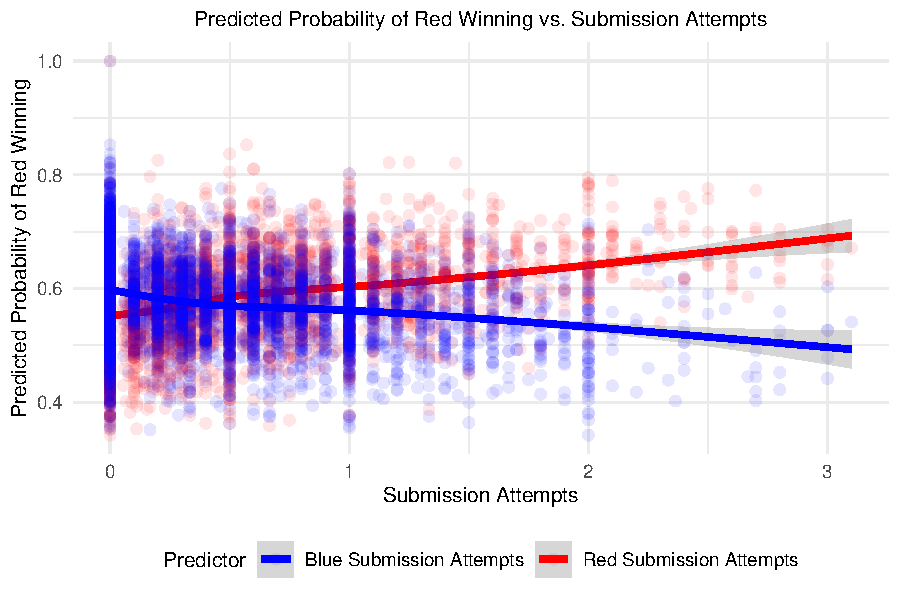
\includegraphics[keepaspectratio]{ufc_final_files/figure-pdf/unnamed-chunk-16-1.pdf}}

This plot visualizes the relationship between submission attempts and
the predicted probability of the red fighter winning in a UFC fight,
with a focus on both the red and blue fighters' submission attempts.
Each point represents an observation, while the red and blue lines
represent logistic regression trends for Red Submission Attempts and
Blue Submission Attempts, respectively.

The upward trend of the red line suggests that as the number of
submission attempts by the red fighter increases, the predicted
probability of the red fighter winning also increases. This aligns with
the odds ratio of 1.548, indicating that each additional submission
attempt by the red fighter significantly improves their chances of
victory.

Conversely, the downward slope of the blue line reveals a negative
relationship for blue fighter submission attempts. As the number of
submission attempts by the blue fighter increases, the predicted
probability of the red fighter winning also increases, suggesting that
blue's submission attempts are ineffective or even counterproductive in
this context. This trend supports the odds ratio of 0.709, showing that
additional submission attempts decrease the odds of the blue fighter
winning.

To summarize, this plot highlights a contrasting effect: while
submission attempts by the red fighter are positively associated with
victory, submission attempts by the blue fighter appear to have the
opposite effect. This difference may reflect strategic or performance
disparities between the fighters, influencing their likelihood of
success.

\subsection{Appendix: Supplementary Materials for UFC
Analysis}\label{appendix-supplementary-materials-for-ufc-analysis}

\textbf{Appendix 1: Diagnostic Plots for Initial Model (Research
Question 1)}

The following diagnostic plots were generated for the initial multiple
linear regression (MLR) model used to explore the relationship between
reach and strikes landed in Research Question 1. These plots highlight
key assumptions of linear regression, including linearity, normality of
residuals, and homoscedasticity.

\pandocbounded{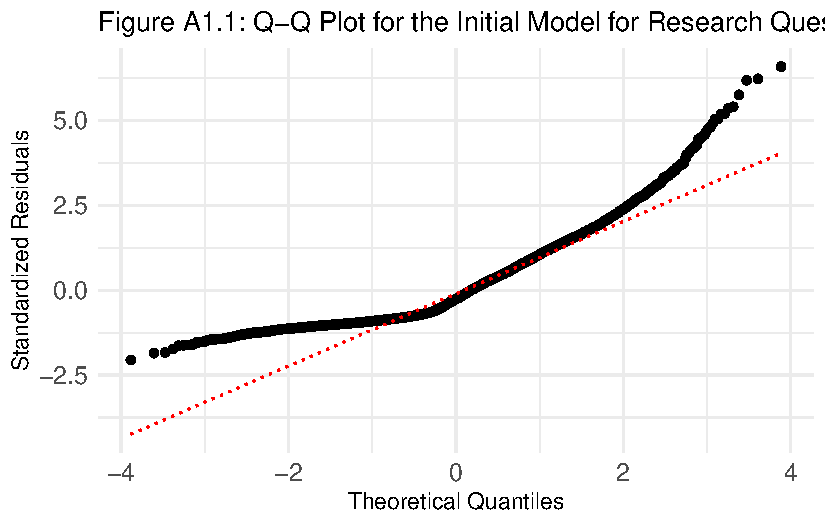
\includegraphics[keepaspectratio]{ufc_final_files/figure-pdf/unnamed-chunk-17-1.pdf}}

\textbf{Appendix 2: Model summaries with AIC score progression (Research
Question 2)}

This section presents the progression of the model selection process for
Research Question 2, examining the relationship between submission
attempts, reach, significant strikes, and fight outcomes. The table
includes the Akaike Information Criterion (AIC) values for different
iterations of the logistic regression model during stepwise selection.
The AIC score, which balances model fit and complexity, is used to
determine the optimal combination of predictors for the final model.
Lower AIC scores indicate a better-fitting model.

The progression shows how variables were added or removed during the
stepwise selection process, highlighting the impact of each predictor on
model performance.

\begin{verbatim}

Call:
glm(formula = Outcome ~ LogRedSubAttempts + LogBlueSubAttempts + 
    LogBlueReach + LogRedReach + LogBlueSigStr + LogRedSigStr + 
    LogFightTime + WeightClass, family = binomial, data = ufc_q2)

Coefficients:
                                  Estimate Std. Error z value Pr(>|z|)    
(Intercept)                      -5.351057   6.459545  -0.828 0.407447    
LogRedSubAttempts                 0.405680   0.089319   4.542 5.57e-06 ***
LogBlueSubAttempts               -0.292197   0.084704  -3.450 0.000561 ***
LogBlueReach                     -1.439347   0.907894  -1.585 0.112883    
LogRedReach                       2.491817   0.903558   2.758 0.005819 ** 
LogBlueSigStr                    -0.365003   0.048374  -7.545 4.51e-14 ***
LogRedSigStr                      0.373853   0.050081   7.465 8.33e-14 ***
LogFightTime                      0.035227   0.032697   1.077 0.281313    
WeightClassCatch Weight          -0.057436   0.343726  -0.167 0.867293    
WeightClassFeatherweight         -0.027917   0.131144  -0.213 0.831425    
WeightClassFlyweight             -0.003566   0.159466  -0.022 0.982161    
WeightClassHeavyweight           -0.045397   0.208875  -0.217 0.827942    
WeightClassLight Heavyweight     -0.176252   0.192860  -0.914 0.360776    
WeightClassLightweight           -0.136914   0.126242  -1.085 0.278128    
WeightClassMiddleweight          -0.276099   0.164307  -1.680 0.092883 .  
WeightClassWelterweight          -0.281531   0.145431  -1.936 0.052888 .  
WeightClassWomen's Bantamweight  -0.177841   0.191071  -0.931 0.351979    
WeightClassWomen's Featherweight  0.230400   0.512452   0.450 0.652996    
WeightClassWomen's Flyweight     -0.122585   0.184749  -0.664 0.506998    
WeightClassWomen's Strawweight    0.011955   0.187268   0.064 0.949100    
---
Signif. codes:  0 '***' 0.001 '**' 0.01 '*' 0.05 '.' 0.1 ' ' 1

(Dispersion parameter for binomial family taken to be 1)

    Null deviance: 6674.5  on 4894  degrees of freedom
Residual deviance: 6566.3  on 4875  degrees of freedom
AIC: 6606.3

Number of Fisher Scoring iterations: 4
\end{verbatim}

\pandocbounded{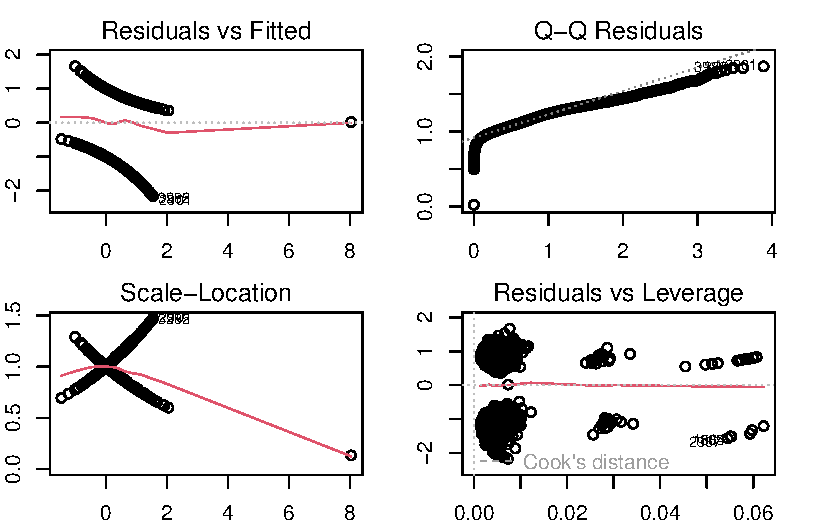
\includegraphics[keepaspectratio]{ufc_final_files/figure-pdf/unnamed-chunk-18-1.pdf}}

\begin{verbatim}

Call:
glm(formula = Outcome ~ LogRedSubAttempts + LogBlueSubAttempts + 
    LogBlueReach + LogRedReach + LogBlueSigStr + LogRedSigStr, 
    family = binomial, data = ufc_q2)

Coefficients:
                   Estimate Std. Error z value Pr(>|z|)    
(Intercept)         0.36477    2.73096   0.134 0.893744    
LogRedSubAttempts   0.39057    0.08768   4.454 8.41e-06 ***
LogBlueSubAttempts -0.29815    0.08385  -3.556 0.000377 ***
LogBlueReach       -1.90853    0.71404  -2.673 0.007521 ** 
LogRedReach         1.88597    0.69892   2.698 0.006967 ** 
LogBlueSigStr      -0.36729    0.04821  -7.618 2.57e-14 ***
LogRedSigStr        0.36873    0.04979   7.405 1.31e-13 ***
---
Signif. codes:  0 '***' 0.001 '**' 0.01 '*' 0.05 '.' 0.1 ' ' 1

(Dispersion parameter for binomial family taken to be 1)

    Null deviance: 6674.5  on 4894  degrees of freedom
Residual deviance: 6577.8  on 4888  degrees of freedom
AIC: 6591.8

Number of Fisher Scoring iterations: 4
\end{verbatim}

\begin{longtable}[t]{lrrrl}
\caption{Logistic Regression Model Coefficients}\\
\toprule
Predictor & Estimate & Std. Error & Z Value & P Value\\
\midrule
Intercept & 0.681 & 2.876 & 0.237 & 0.813\\
Log Red Submission Attempts & 0.437 & 0.097 & 4.494 & <0.001\\
Log Blue Submission Attempts & -0.343 & 0.094 & -3.660 & <0.001\\
Log Blue Reach & -2.108 & 0.766 & -2.752 & 0.006\\
Log Red Reach & 2.030 & 0.743 & 2.732 & 0.006\\
\addlinespace
Log Blue Significant Strikes & -0.468 & 0.057 & -8.201 & <0.001\\
Log Red Significant Strikes & 0.462 & 0.059 & 7.876 & <0.001\\
\bottomrule
\end{longtable}

\begin{longtable}[t]{rrrrr}
\caption{Model Fit Statistics}\\
\toprule
Null Deviance & DF Null & Residual Deviance & DF Residual & AIC\\
\midrule
6323.988 & 4643 & 6221.674 & 4637 & 6235.674\\
\bottomrule
\end{longtable}

\pandocbounded{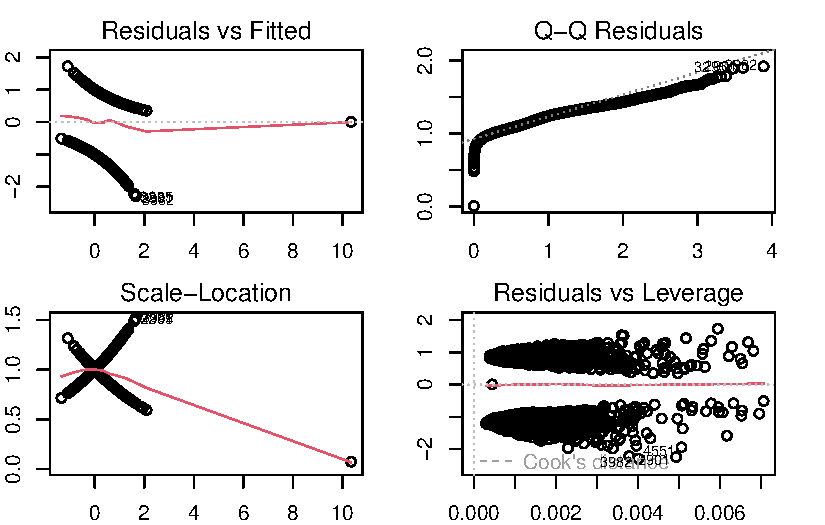
\includegraphics[keepaspectratio]{ufc_final_files/figure-pdf/unnamed-chunk-18-2.pdf}}




\end{document}
